\documentclass[10pt, oneside]{article} 
\usepackage{amsmath, amsthm, amssymb, wasysym, verbatim, bbm, color, graphics, geometry,
  hyperref, biblatex, mathtools}
\usepackage[framemethod=TikZ]{mdframed}
\usepackage{tcolorbox}

\hypersetup{
	colorlinks=true,
	linkcolor=blue,
	urlcolor=blue
}

\addbibresource{ref.bib}

\geometry{tmargin=.75in, bmargin=.75in, lmargin=1.25in, rmargin=1.25in}
\setlength\parindent{0pt}

\tcbuselibrary{theorems}
\newtcbtheorem
    []% init options
    {problem}% name
    {Problem}% title
    {%
      fonttitle=\bfseries,
    }% options
    {prob}% prefix

    \newcommand{\R}{\mathbb{R}}
    \newcommand{\C}{\mathbb{C}}
    \newcommand{\Z}{\mathbb{Z}}
    \newcommand{\N}{\mathbb{N}}
    \newcommand{\Q}{\mathbb{Q}}
    \newcommand{\Cdot}{\boldsymbol{\cdot}}

    \newtheorem{thm}{Theorem}
    \newtheorem{defn}{Definition}
    \newtheorem{conv}{Convention}
    \newtheorem{rem}{Remark}
    \newtheorem{lem}{Lemma}
    \newtheorem{cor}{Corollary}
    \newtheorem{prop}{Proposition}

    \newcommand{\tr}{\mathrm{Tr}}


    \title{When MAT240 Gets Confusing...}
    \author{Jack Ceroni}
    \date{December 2020}

    \begin{document}

    \maketitle
    \tableofcontents

    \vspace{.25in}

    \newpage

    \section{Introduction}

    I do spend a little bit of time discussing concepts that any reader (who took MAT240) will likely already
    be familiar with (invariant subspaces, eigenspaces, etc.), but I want to keep these notes fairly self-contained.
    \newline

    If you notice any mistakes in these notes, please do not hesitate to send me an email or
    send me a message on the Math Physics Specialist Discord server.

    \section{What Are These Notes About?}

    These notes are meant to sequentially explain how we go about understanding linear operators on vector
    spaces by ``breaking them up'' into simpler, more understandable pieces, choosing a nice basis for
    each of these peices, and then putting them back together.
    \newline

    Formally, these concepts are know as the \textbf{decomposition theorem} and \textbf{Jordan Canonical Form}.

    \section{Invariant Subspaces}

    Before we begin our discussion of the decomposition theorem, we
    first must briefly cover the idea of \textbf{invariant subspaces}.
    Simply put, an invariant subspace $U$ is a subspace
    of the vector space $V$ that behaves ``nicely'' under an operator $T$ on $V$.
    \newline

    More specifically:

    \begin{defn}
      An invariant subspace in defined as a subspace $U$ of $V$ such that if $u \in U$, then $Tu \in U$.
      \end{defn}

      A consequence of this definition is that the operator $T |_{U} \in \mathcal{L}(U)$: the restriction
      of $T$ to the domain $U$ inside of $V$ is well-defined (consider the alternative, if $U$ wasn't invariant then
      there would exist some $u \in U$ that gets
      sent somewhere outside of $U$ by $T|_U$, so $T|_U$ wouldn't be a valid map from $U$ to $U$).

      \begin{center}
        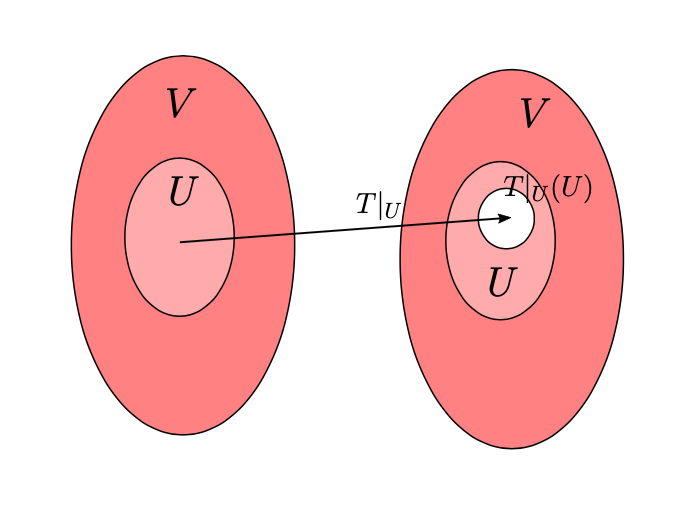
\includegraphics[width=200pt]{assets/invar.png}
      \end{center}

      \section{Eigenvalues and Eigenvectors}

      Now that the idea of an invariant subspace has been introduced, we can discuss some simple examples
      of invariant subspaces.
      \newline

      Given an operator $T$, some fairly obvious examples of spaces that are invariant are $\text{Null} \ T$ and
      $\text{Range} \ T$. However, let's consider an even simpler example: a one-dimensional invariant subspace.
      \newline

      Let $U$ be a one-dimensional invariant subspace. Clearly, there is only one linearly independent
      vector $u \in U$, so $U$ is the space of all vectors of the form $c u$, for $c \in \mathbb{F}$.
      \newline

      Since $T$ is invariant, we must then have $T(u) = \lambda u$ for some $\lambda \in \mathbb{F}$.
      It then follows that for any other $cu$
      in $U$, we will have $T(cu) = cT(u) = c\lambda u = \lambda(cu)$.
      \newline

      We call $\lambda$ an \textbf{eigenvalue} of $T$, and all the vectors in $U$ \textbf{eigenvectors} of $T$
      corresponding to $\lambda$.
      \newline

      Intuitively, eigenvectors of $T$ are vectors such that that $T$ sends them to a scalar multiple
      of themself, and the eigenvalues are these correspionding scalar multiples.

      \begin{center}
        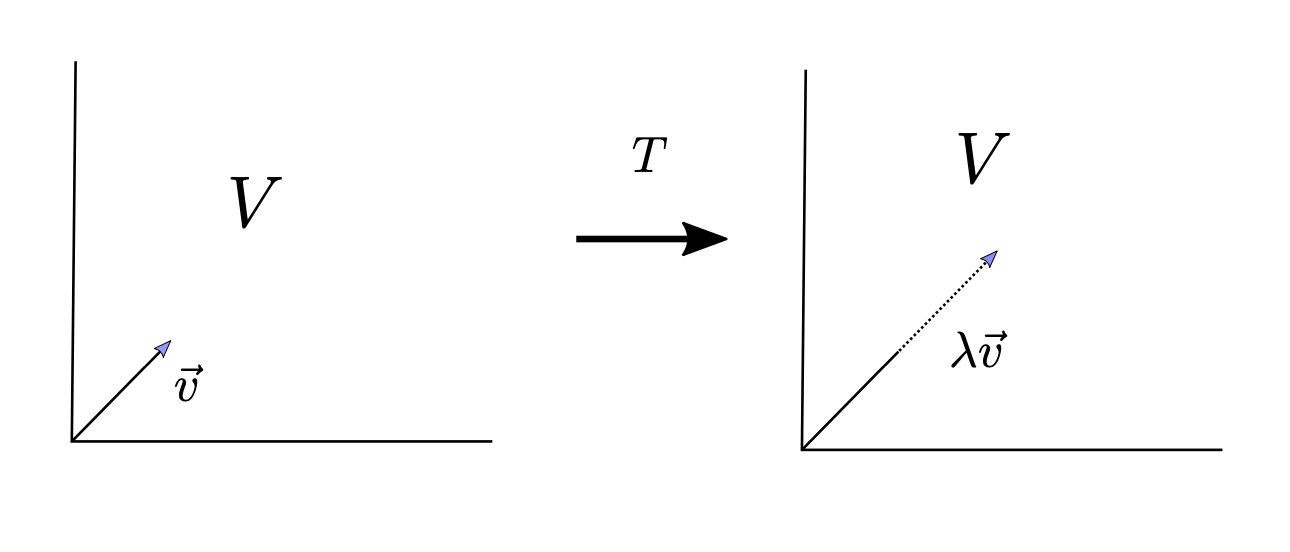
\includegraphics[width=300pt]{assets/eig.png}
      \end{center}

      Before we proceed any further, we stop to prove a very important result about eigenvectors:

      \begin{prop}
      Given a set of $m$ distinct eigenvalues $\lambda_1, \ ..., \ \lambda_m$, along with a set of corresponding eigenvectors $V = \{v_1, \ ..., \ v_m\}$, the
      set $V$ is linearly independent.
    \end{prop}

    \begin{proof}

      We will prove this proposition by induction. Clearly, this will be true in the case of one eigenvalue, $\lambda$. Assume that
      it holds true given $n$ eigenvalues. We prove it holds true for $n + 1$.
      \newline

      Consider the set of eigenvalues $\{\lambda_1, \ ..., \ \lambda_{n + 1}\}$ with
      corresponding eigenvectors $\{v_1, \ ..., \ v_{n + 1}\}$.
      Assume that there is a non-trivial linear combination:

      $$a_{1} v_1 + \ \cdots \ + a_{n} v_{n} + a_{n + 1} v_{n + 1} = 0$$

      Note that since eigenvectors are non-zero, for this non-trivial linear combination to be $0$, we must have at least two $a_i$ not equal to
      $0$ otherwise we would have $a_k v_k = 0$, for non-zero $a_k$, which can't be the case. It follows that at least one $a_i$ with $1 \leq i \leq n$
      is non-zero.
      \newline

      We define the linear operator $(T - \lambda_{n + 1} I)$. We then have:

      $$(T - \lambda_i I)(a_1 v_1 + \ \cdots \ + a_n v_n + a_{n + 1} v_{n + 1}) = \displaystyle\sum_{k \neq n + 1} a_k (\lambda_k - \lambda_{n + 1}) v_k = 0$$

      But since all eigenvalues are unique, we must have $\lambda_k - \lambda_{n + 1} \neq 0$. In addition, it least one $a_i$ in this sum is non-zero. Thus,
      we have found a non-trivial linear combination of $n$ eigenvectors that yields the zero vector, a contradiction to the inductive hypothesis.
      \newline

      It follows that the set $\{v_1, \ ..., \ v_{n + 1}\}$ is linearly independent and the proof is complete.

    \end{proof}

    \begin{cor}
      Given some finite-dimensional
      $V$ and some $T \in \mathcal{L}(V)$, $T$ can have at most $\dim \ V$ distinct eigenvalues.
    \end{cor}

    \begin{proof}
      Assume we had more than $\dim \ V$ eigenvalues. We would then have a set of more than $\dim \ V$
      linearly independent eigenvectors, a clear contradiction.
      \end{proof}

    \begin{cor}
      Given a vector space $V$ of dimension $n$ and some $T \in \mathcal{L}(V)$,
      if there exist $n$ distinct eigenvalues $\lambda_1, \ ..., \ \lambda_n$, then there exists a
      basis of $V$ composed of eigenvectors.
    \end{cor}

    \subsection{Eigenspaces}

    Given the fact that we are interested in invariant subspaces, we formalize the notion of a
    collection of eigenvectors,
    which we know from above is an invariant subspace:

      \begin{defn}
     Given some operator $T \in \mathcal{L}(V)$ and some eigenvalue $\lambda$ of $T$,
     An \textbf{eigenspace} of $T$ is defined to be the
     subspace $E(\lambda, \ T)$ of $V$ containing the eigenvectors associated to $\lambda$.
   \end{defn}

   Note that from the definition, it is clear that:

   $$E(\lambda, \ T) = \text{Null} \ (T - \lambda I)$$

   As it will turn out, eigenspaces are very powerful
     
      \section{The Decomposition Theorem}

      \subsection{Motivation}

    Consider some operator $T \in \mathcal{L}(V)$, where $V$ is finite-dimensional.
    \newline

    In general, it is easier to make sense of linear maps if we can break them up
    into many pieces, which we can then analyze separately. Intuitively, if we can
    come up with a collection of subspaces $V_1, \ ..., \ V_n$ such that each has a ``simple''
    structure and:

    $$V = V_1 \oplus V_2 \oplus \ \cdots \ \oplus V_n$$

    then it is possible that consider $T$ acting on each individual $V_k$ might give some insight
    into the underlying structure of $T$.
    \newline

    But, under what circumstances can we do this? Well, if we want to understand how $T$ acts on
    each individual $V_k$, then we should consider $T$ restricted to the domain $V_k$, which we denote $T|_{V_k}$.
    However, $T|_{V_k}$ isn't always well-defined. As we explained in Section 2, such restrictions only
    ``make sense'' when $V_k$ is an \textbf{invariant subspace}.
    \newline

    Thus, we want to find subspaces $V_k$ that are \textbf{invariant} under $T$.

    \subsection{Eigenspaces}

    Now that we know what we are looking for (invariant subspaces whose direct sum is equal to $V$), we
    can start thinking about what these invariant subspaces should actually be.

    One of the most familiar examples of an invariant subspace that the reader of these notes is likely familiar 


    \subsection{Operators and Polynomials}

    The main idea of this section is to write $V$ is a convenient way, in terms of its eigenvalues.
    \newline



   \subsection{The Decomposition Theorem}

   \begin{defn}
     Given some operator $T \in \mathcal{L}(V)$ and some eigenvalue $\lambda$ of $T$,
     An \textbf{eigenspace} of $T$ is defined to be the
     subspace $E(\lambda, \ T)$ of $V$ containing the eigenvectors associated to $\lambda$.
   \end{defn}

   Note that from the definition, it is clear that:

   $$E(\lambda, \ T) = \text{Null} \ (T - \lambda I)$$

   \begin{defn}
     Generalized eigenvectors and eigenspaces
   \end{defn}

   \begin{lem}
     $V$ is the null space of the product
   \end{lem}

   \begin{lem}
     The sum of the null spaces is direct
     \end{lem}

   \begin{lem}
     Given two operators $S$ and $T$ in $\mathcal{L}(V)$, where $V$ is finite-dimensional, then:

     $$\dim \ \mathrm{Null} \ ST = \dim \ \mathrm{Null} \ T + \dim \ (\mathrm{Range} \ T \cap \mathrm{Null} \ S)$$
   \end{lem}

   For some intuition as to why this is true, consider the following diagram:

   \begin{center}
     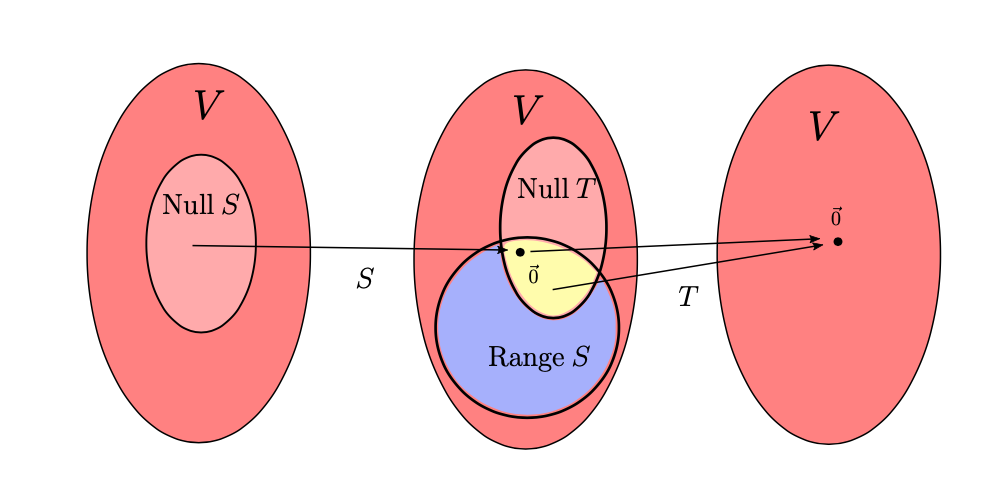
\includegraphics[width=300pt]{assets/map.png}
   \end{center}

   Clearly, only vectors in the left-most null space and the yellow region get sent to the zero vector,
   after we ``apply'' the maps $S$ and then $T$ to $V$.
   \newline

   If you look closer, you will notice that
   these two regions are exactly $\text{Null} \ T$ and $\text{Range} \ T \cap \ \text{Null} \ S$ respectively!

   \begin{lem}
     Necessary result to prove this.
     \end{lem}

   \begin{proof}

   \end{proof}

   \begin{prop}
     The null space of the product is equal to the direct sum of all the null spaces
   \end{prop}

   This allows us to conlude that we can decompose $V$.

   \section{Upper Triangular Matrices}

   \begin{prop}
     Every operator over $\mathbb{C}$ on a finite-dimensional vector space has an upper-triangular matrix representation in some basis.
   \end{prop}

   \begin{proof}

     This is clearly true when $T$ is an operator on a vector space of dimension $1$. Now, assume that this proposition holds true
     in the case of a vector space $V$ with $\dim \ V = n$. We prove the case of $n + 1$.
     \newline

     Since the vector space is over the complex field, we choose an eigenvalue $\lambda$. We consider the invariant subspace:

     $$U = \text{range} (T - \lambda I)$$

     Since $T - \lambda I$ is not injective, it is not surjective, so $\dim \ U < \dim \ V$. By our inductive hypothesis, we choose a
     basis $u_1, \ ..., \ u_m$ of $U$ that puts $T|_{U}$ in upper triangular form. Then, we extend the list $u_1, \ ..., \ u_m$ to a basis
     by adding $v_1, \ ..., \ v_k$, and note that:

     $$Tv_j = (T - \lambda I)v_j + \lambda v_j$$

     so $v_j$ is a sum of an element of $U$, and a multiple of $v_j$ itself. Thus, $Tv_j \in \text{span}(u_1, \ ..., \ u_m, \ v_1, \ ..., \ v_j)$.
     It follows by definition that our new basis puts $T$ in upper triangular form.

     \end{proof}

   \begin{lem}
     An operator $T$ on $V$ is invertible if and only if all the entries on the diagonal of an
     upper-triangular representation of $T$ are non-zero.
     \end{lem}

   \begin{cor}
     The eigenvectors of some operator $T$ on $V$ are the diagonal elements of an
     upper-triangular matrix representation of $T$
     \end{cor}

   \section{Jordan Canonical Form}

   \subsection{Sending Lemmings Off the Cliff: Finding the Jordan Basis}

   Now comes arguably the most confusing part of the notes: defining a basis that puts some operator
   $T \in \mathcal{L}(V)$ in Jordan form. We will attempt to explain each step using diagrams, to help
   with conceptualizing all of the choices we make.
   \newline

   To briefly recap, we know that given some vector space $V$ and some $T \in \mathcal{L}(V)$, we will have:

   $$V = c \displaystyle\prod_{k = 1}^{n} \text{Null} \ (T - \lambda_k I)^{m_k}$$

   for sets $\lambda_1, \ ..., \ \lambda_n$ and $m_1, \ ..., \ m_n$. Using this fact, we proved the
   decomposition theorem, showing that:

   $$V = \text{Null} \ (T - \lambda_1 I)^{m_1} \oplus \ \cdots \ \oplus \text{Null} \ (T - \lambda_n I)^{m_n}$$

   We are trying to find a convenient basis. With the above fact, it follows that we only have to
   find a convenient basis \textbf{for each} $\text{Null} \ (T - \lambda_1 I)^{m_1}$.
   Then, since the sum of these subspaces is direct,
   we can combine all of our ``nice'' bases, giving us a ``nice'' basis for the whole vector space $V$.
   \newline

   Hopefully this example illuminates why decomposing $V$ into a collection of simpler pieces is useful in
   the first place!

   \subsubsection{Finding a Basis for Each Invariant Subspace}

   Let us consider some component of our vector space, of the form $U = \text{Null} \ (T - \lambda_k I)^{m_k}$.
   \newline

   By definition of this space, given some $u \in U$, it follows that $u$ must be sent to $0$ by $(T - \lambda_k I)^{m_k}$:
   However,
   there are a lot of different ways this could happen. For instance, if $m_k = 3$, then we must have:

   $$(T - \lambda_k I) (T - \lambda_k I) (T - \lambda_k I) v = 0$$

   so hypothetically, $v$ could be sent to $0$ be the first application of $(T - \lambda_k I)$, the second or the third. In other words,
   we could have $(T - \lambda_k I) v = 0$, $(T - \lambda_k I)^2 v = 0$, or $(T - \lambda_k I)^3 v = 0$.
   \newline

   More generally given some $m_k$, some
   $v \in U$ will be sent to $0$ for some least $k \leq m_k$, and then will also be sent to $0$ be all subsequent $k$, as a linear map applied to $0$ is still $0$.
   \newline

   PIC
   \newline

   This fact gives us an interesting way to find a nice-looking basis for $U$. Let $e_1, \ ..., \ e_n$ be some arbitrary basis of $U$. From above we know that each of
   these basis vectors must be sent to $0$ by repeatedly applying $(T - \lambda_k I)$ some number of times. This implies that there is a natural way that we can
   ``split up'' our basis into different subsets, based
   on the \textbf{smallest number of times} we have to apply $(T - \lambda_k I)$ to get the $0$ vector.
   \newline

   For instance, in the case of $m_k = 3$, maybe we will have three basis vectors $e_1$, $e_2$ and $e_3$, where $e_1$ and $e_3$ get sent to $0$ with one application of $(T - \lambda_k I)$, while
   $e_2$ gets sent to $0$ by two applications of $(T - \lambda_k I)$, but does not get sent to $0$ by only one application.
   \newline

   Note that since $e_2$ \textbf{doesn't} get sent to $0$ by
   one application of $(T - \lambda_k I)$, it follows that the vector $(T - \lambda_k I)(v)$ is non-zero, and will get sent to $0$ by \textbf{one} application of $(T - \lambda_k I)$. Therefore,
   we can conclude that $(T - \lambda_k I)(v)$ must be a linear combination of $e_1$ and $e_3$ (the basis vectors that get sent to $0$ be one application of $(T - \lambda_k I)$). In fact, the
   null spaces of the operators will looking something like this:
   \newline

   PIC
   \newline

   As you may have guessed, this method gives us nice way to look for a matrix in Jordan form. Recall that a matrix of some operator in Jordan form looks something like this:
   \newline

   PIC
   \newline

   Where each ``block'' is called a \textbf{Jordan block}. 

    \end{document}
